\chapter{Конструкторский раздел}
\label{design}
\section{Структура разрабатываемого программного обеспечения}
	Для создания разрабатываемого программного обеспечения необходимо реализовать:
\begin{itemize}
\item Загружаемый модуль ядра.
\item Пользовательское приложение.
\end{itemize}

	Согласно поставленной задачи, пользователь должен осуществлять управление мышью через Android устройство удаленно, поэтому пользовательское приложение необходимо реализовать в виде клиент-серверного приложения. Таким образом, пользовательское приложение будет состоять из двух частей: программы сервера и программы клиента.
\begin{itemize}
\item Клиент - приложение, разработанное для Android устройства, которое предоставляет ползователю осуществлять управление мышью.
\item Сервер - приложение, работающее на ПК в фоновом режиме, отвечающее за получение данных от клиентского приложения и передачу их загружаемому модулю ядра.
\end{itemize}

	Передача данных между смартфоном и ПК будет осуществляться с помощью протокола RFCOMM\cite{btprotocol}. Он используется L2CAP\cite{btprotocol} (базовый протокол передачи данных для Bluetooth) в качестве транспортного. Основной принцип действия заключается в эмулировании соединения point-to-point по последовательному порту. В связи с этим структура программного обеспечения будет выглядеть, как на рисунке~\ref{fig: view_struct}.
	
\begin{figure} [h!]
  \centering
  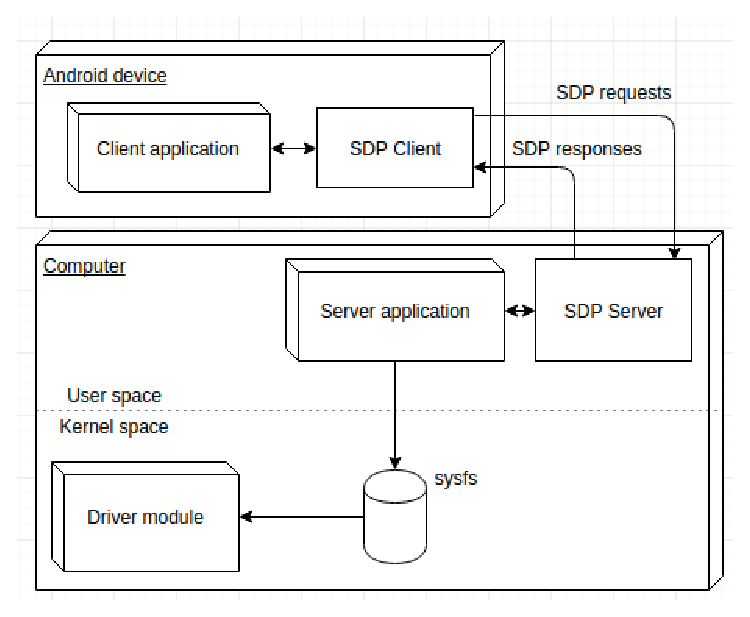
\includegraphics[scale=0.75]{design/structure}
  \caption{Структура программного обеспечения}
  \label{fig: view_struct}
\end{figure}
\label{driver}
\section{Загружаемый модуль ядра}
	Загружаемый модуль ядра должен решать следующие задачи:
\begin{itemize}
\item Чтение данных из пространства ядра.
\item Регистрация устройства в подсистеме ввода ядра.
\end{itemize}

	Обмен данными между пространством ядра и пространством пользователя происходит при помощи виртуальной файловой системы в ОС Linux - \texttt{sysfs}~\cite{ldd3}. В \texttt{Sysfs} имеется подкаталог, где содержится вся информация о перифирийных подключаемых устройствах, присущих конкретной платформе. Все, что необходимо для обмена: создать в этом самом подкаталоге \texttt{/sys/devices/platform}, каталог с файлом, в который сервер будет записывать поступающие данные от Android приложения. Данный каталог создается командой \Code{command\_result = sysfs\_create\_group(\&vms\_dev->dev.kobj, \&vms\_attr\_group);}.
	
	При обмене информацией между всеми приложениями необходимо определить содержание и формат передаваемых данных. Для корректной работы мыши, загружаемый модуль должен получать текущие координаты положения курсора и тип команды. Передаваемые данные запишем в виде строки, состоящей из 4 чисел:
\begin{itemize}
\item Команда
\item Координата курсора мыши по оси X
\item Координата курсора мыши по оси Y
\item Координата курсора мыши по оси Z
\end{itemize}

Также, необходимо сразу уточнить, какие команды могут подаваться от устройства:
\begin{itemize}
\item Перемещение курсора
\item Нажатие левой клавиши мыши
\item Нажатие правой клавиши мыши
\item Двойной щелчок левой клавиши мыши
\end{itemize}

	Регистрация устройства происходит по следующим этапам:
\begin{enumerate}
\item Регистрация платформо зависимого устройства в системе.
\item Создание файла устройства в \Code{sysfs}.
\item Выделение памяти под устройство ввода.
\item Установка обработчика на события.
\item Регистрация устройства в подсистеме ввода.
\end{enumerate}
\vspace{1.4cm}

\begin{lstlisting}[style=pseudocode,caption={Алгоритм регистрации устройства в системе}]
def display_init(void):
    command_result = 0;

    vms_dev := platform_device_register_simple("vms", -1, NULL, 0)
    if (IS_ERR(vms_dev)) 
        PTR_ERR(vms_dev)
        printk("vms_init: error\n")
        return ERROR_REGISTER_PLATFORM_DEVICE

    command_result := sysfs_create_group(vms_dev->dev.kobj, vms_attr_group);
    
    if (command_result < 0)
        printk("Error sysfs_create_group\n")
        return ERROR_SYSFS_CREATE_GROUP

    vms_input_dev := input_allocate_device()
    if (!vms_input_dev) 
        printk("Bad input_alloc_device()\n")
        return ERROR_ALLOCATE_INPUT_DEVICE

    set_bit(EV_REL, vms_input_dev->evbit)
    set_bit(REL_X, vms_input_dev->relbit)
    set_bit(REL_Y, vms_input_dev->relbit)
    set_bit(EV_KEY, vms_input_dev->evbit)
    set_bit(BTN_LEFT, vms_input_dev->keybit)
    set_bit(BTN_RIGHT, vms_input_dev->keybit)

    vms_input_dev->evbit[0] := BIT_MASK(EV_KEY) | BIT_MASK(EV_REL)
    vms_input_dev->keybit[BIT_WORD(BTN_MOUSE)] := BIT_MASK(BTN_LEFT) |
        BIT_MASK(BTN_MIDDLE) | BIT_MASK(BTN_RIGHT)
    vms_input_dev->relbit[0] := BIT_MASK(REL_X) | BIT_MASK(REL_Y)

    vms_input_dev->name := "Virtual BT mouse"
    vms_input_dev->id.bustype := BUS_VIRTUAL
    vms_input_dev->id.vendor  := 0x0000
    vms_input_dev->id.product := 0x0000
    vms_input_dev->id.version := 0x0000
    
    command_result := input_register_device(vms_input_dev)
    
    if (command_result < 0)
        printk("Error input_register_device\n")
        return ERROR_REGISTER_INPUT_DEVICE
  
    printk("Virtual BT Mouse Driver Initialized.\n")
    return 0
\end{lstlisting}

\label{sec: android}
\section{Приложение для Android устройства}
	Клиентское приложение уровня пользователя должно осуществлять обработку запросов пользователя, установку соединения с серверным приложением и последующую передачу данных.

	Для установки соединения с сервером необходимо использовать Bluetooth API~\cite{btandroid}. Работа с bluetooth происходит в 4 этапа:
\begin{enumerate}
\item Инициализация адаптера.
\item Поиск доступного сервера.
\item Установка соединения.
\item Передача данных.
\end{enumerate} 
	
	Инициализация адаптера происходит с помощью функции \Code{BluetoothAdapter.getDefaultAdapter()}. Передача данных осуществляется при помощи сокетов. Сокет - это название программного интерфейса для обеспечения обмена данными между процессами\cite{socket}. Процессы при таком обмене могут исполняться как на одной ЭВМ, так и на различных ЭВМ, связанных между собой сетью. Сокет — абстрактный объект, представляющий конечную точку соединения. Ниже представлен алгоритм подключения к серверу:
\begin{lstlisting}[style=pseudocode,caption={Алгоритм подключения к серверу}]
def connectToServer():
	device := adapter.getRemoteDevice(SERVER_MAC_address)
	socket := device.createRfcommSocketToServiceRecord(SERVER_UUID)
	adapter.cancelDiscovery()
    socket.connect()
	stream := socket.getOutputStream()
\end{lstlisting}

	Для передачи данных мы используем выходной поток \Code{stream}, созданный при подключении.
\vspace{1.2cm}
\begin{lstlisting}[style=pseudocode,caption={Алгоритм передачи данных}]
def sendDataToServer():
	buffer := msg.getBytes()
	if (stream != null)
		stream.write(buffer)
\end{lstlisting}
	
\label{server}
\section{Сервер}
	Серверное приложение уровня пользователя должно решать следующие задачи:
\begin{itemize}
\item Установка соединения с клиентским приложением.
\item Получение данных от клиентского приложения.
\item Передача данных в пространство ядра.
\end{itemize}

	Установка соединения с клиентским приложением осуществляется по алгоритму 2.1. Перед запуском сервера~\cite{bluez} необходимо установить уникальный UUID - 16-байтный номер, используемый для уникальной идентификации сервера. Кроме того, требуется установить значение порта.  
\begin{lstlisting}[style=pseudocode,caption={Алгоритм запуска сервера}]
def startServer():
	server.socket := BluetoothSocket(RFCOMM)
	server.socket := bind("",server.port)
	server.socket := listen(server.port)
	
    advertise_service( server.socket, server.name, 
    	service_id := server.uuid,
		service_classes := [ server.uuid, SERIAL_PORT_CLASS ],
		profiles = [ SERIAL_PORT_PROFILE ]
		)
		
	print("Waiting a client...")
	
	client.socket, client.info := server.socket := accept()
\end{lstlisting}

	После запуска, сервер находится в ожидании подключения клиента. Как только один из клиентов подал правильный sdp-запрос, сервер переходит в бесконечный цикл для приема данных от клиента и последующей записи в пространство ядра. 
\vspace{1.2cm}
\begin{lstlisting}[style=pseudocode,caption={Алгоритм передачи данных в пространство ядра}]
def sendData():
	while True:
        data := client.socket := recv(size)
        if len(data) == 0: break
        os.write(fd, data) # fd - file created by the driver for the adoption of the coordinates
        os.fsync(fd)
        if "</EOM>" in data: break
\end{lstlisting}
	
	Как только клиент отправил запрос об окончании передачи данных, сервер отправляет ответное сообщение о закрытии подключения и закрывает сначала клиентский сокет, а затем и свой.
		
\begin{lstlisting}[style=pseudocode,caption={Закрытие подключения}]
def stopServer():
	client.socket := send("The server will be turned off soon")

	client.socket := close()
	server.socket := close()
\end{lstlisting}

%%% Local Variables: debug
%%% mode: latex
%%% TeX-master: "rpz-os"
%%% End: